\documentclass{article}
\usepackage[top=2cm, bottom=2cm, left=2.2cm, right=2.5cm]{geometry}
\usepackage{amsmath,amsfonts,amssymb,amsthm}
\usepackage{enumerate}% http://ctan.org/pkg/enumerate

\usepackage[]{pdfcomment}
%As recommended by matlab2tikz
\usepackage{pgfplots}
\usepackage{tikz}
\usepackage{nicematrix}
\usepackage{calc}
\usepackage{pgfplotstable}
\usepackage{booktabs}
\usepackage{csvsimple}
\usepackage{etoolbox}
\usepackage[style=alphabetic]{biblatex}
\usepackage{amsthm}
\bibliography{refs.bib}
%% the following commands are needed for some matlab2tikz features
\usetikzlibrary{plotmarks}
\usetikzlibrary{arrows.meta}
\usepgfplotslibrary{patchplots}
\usepackage{grffile}
%% you may also want the following commands
\pgfplotsset{plot coordinates/math parser=false}
%\newlength\figureheight
%\newlength\figurewidth
\usepackage{hyperref}
\usepackage{placeins,nicefrac}
\usepackage{xstring}
\usepackage[]{pgfkeys}
\usepackage{xfrac}
\usepackage{breqn}%dmath, might be problematic sometimes
\usepackage[newfloat]{minted}
\usetikzlibrary{external}
\usetikzlibrary{calc,math}
\tikzexternalize[prefix=extern/]
\usepgfplotslibrary{groupplots}
\usepgfplotslibrary{colormaps}
\usetikzlibrary{decorations.markings,decorations.pathreplacing,patterns,patterns.meta,pgfplots.fillbetween}

\usepackage[ruled,vlined,linesnumbered,algo2e]{algorithm2e}
\usepackage{wrapfig}
\usepackage{subcaption}
\newenvironment{code}{\captionsetup{type=listing}}{}
\SetupFloatingEnvironment{listing}{name=Source Code}
\graphicspath{../plots/}

\usepackage{wasysym}
\usepackage{animate}
\usepackage[symbol]{footmisc}

%\usepackage{expl3}
%\ExplSyntaxOn
%\cs_set_eq:NN \fpeval \fp_eval:n
%\ExplSyntaxOff

\usetikzlibrary{fpu}
\graphicspath{{../figs/}}
\newcommand{\figurescale}{1.0}

\newcommand\minput[1]{%
	\input{#1}%
	\ifhmode\ifnum\lastnodetype=11 \unskip\fi\fi}
%\usepackage{titlesec}
%\titleformat{\subsection}{\normalfont\large\bfseries}{Task \thesubsection}{1em}{}
%\titleformat{\section}{\normalfont\Large\bfseries}{Assignment \thesection}{1em}{}
%\titleformat{\subsubsection}{\normalfont\bfseries}{Question \thesubsubsection}{1em}{}
\newcommand\mycommfont[1]{\ttfamily\textcolor{blue}{#1}}
\SetCommentSty{mycommfont}

\newcommand{\stilltodo}[1]{{\color{red} UNFINISHED #1}}

\makeatletter
\newcommand{\trp}{%
	{\mathpalette\@transpose{}}%
}
\newcommand*{\@transpose}[2]{%
	% #1: math style
	% #2: unused
	\raisebox{\depth}{$\m@th#1\intercal$}%
}

\makeatother
\newcommand{\diff}{\mathrm{d}}
\newcommand{\mbf}[1]{\mathbf{#1}}
\author{Andr\'as Schifferer, r0915705}
\title{Numerical Linear Algebra [H03G1A]\\{\LARGE HW2}\\{\large Regularization}}
\date{\today} 

\pgfplotsset{plot coordinates/math parser=false}

\makeatletter
\providecommand{\leftsquigarrow}{%
	\mathrel{\mathpalette\reflect@squig\relax}%
}
\newcommand{\reflect@squig}[2]{%
	\reflectbox{$\m@th#1\rightsquigarrow$}%
}
\makeatother


\newtheorem{lemma}{Lemma}
\newcommand{\lemmaautorefname}{Lemma}
\newtheorem{theorem}{Theorem}
\DeclareMathOperator*{\argmin}{arg\,min} % thin space, limits underneath in displays
\DeclareMathOperator*{\argmax}{arg\,max} % thin space, limits underneath in displays

\begin{document}
	\maketitle
	%The assignment is not yet finished unfortunately.
	\tableofcontents
	
	%%%%%%%%%%%%%%%%%%%%
	\section{Theory}
	%%%%%%%%%%%%%%%%%%%%
	The concept of ill-posedness was first studied by Jacques Hadamard in the beginning of the 20th century. Hadamard essentially defined a problem to be well-posed (“bien posé”) if the solution is unique and if it is a continuous function of the data. Contrary, an ill-posed problem is one that is not
	uniquely solvable or not continuous as a function of the data i.e. if small perturbation of the data can cause large perturbations in the solution.
	The typical example of an ill-posed problem is a Fredholm integral equation of the first kind with a square integrable kernel
	$$g(s)=\int_{a}^{b}K(s,t)f(t) \,d t,\quad c\leq s\leq d$$
	with given K and g, where f is an unknown solution.\\
	There are certain finite-dimensional discrete problems that have properties very similar to those of ill-posed problems, such as being highly sensitive to high frequency perturbations. Examples include the discretizations of the above integral equations. We can be more precise and say that a system of
	the form
	$$A\mathbf{x}=\mathbf{b}, A\in \mathbb{R}^{m\times n}$$
	is a discrete ill-posed problem if both the following conditions are satisfied:
	\begin{itemize}
		\item[1.]the singular values of A decay gradually to zero
		\item[2.]the ratio between largest and smallest singular values is large
	\end{itemize}
	Criterion 2 implies that the matrix A is ill-conditioned, while criterion 1 implies that there is no
	“nearby” problem with a well-conditioned coefficient matrix and with well-determined numerical rank.\\
	Being ill-posed is not a fundamental barrier to systems being solvable. Rather, the ill-conditioning
	means that standard solution procedures are not useful. Indeed, the many small singular values of
	a discrete ill-posed problem essentially make the problem (numerically) under determined. One has
	to resort to more sophisticated methods, incorporating additional information about the solution, in
	order to compute a useful solution. This is the central idea behind regularization methods. When such `side constraints’ are introduced, one must give up the requirement $Ax = \mbf{b}$ exactly in the linear system and instead seek a solution that provides a fair balance between minimizing some cost function that encodes the side constraints and minimizing the residual norm $\|A\mbf{x} -\mbf{b}\|_2$ .\\
	
	The further parts of the assignment use heavily the package by \textcite{regtools}.
	
	\subsection{Tikhonov regularization}
	Undoubtedly, the most common and well-known form of regularization is Tikhonov regularization.
	Here, the idea is to define the regularized solution $\mbf{x}_{\lambda}$ (as a function of $\lambda$) as the minimizer of the following weighted
	combination of the residual norm and a side constraint
	\begin{equation}\label{eq:basicTikh}
		\mbf{x}_{\lambda} = \argmin_{\mbf{x}} \{\|A\mbf{x} - \mbf{b}\|_2^2 + \lambda^2 \|L(\mbf{x} - \mbf{x}^{\ast} )\|_2^2\},
	\end{equation}
	where the regularization parameter $\lambda$ controls the weight given to minimization of the side constraint
	relative to minimization of the residual norm. The side constraint is captured by the matrix $L$. One
	typical example is $L = I_n$ . In this case, a large $\lambda$ (strong regularization) favors a small solution norm at the cost of large residual norm, while a small $\lambda$ has the opposite effect. Other choices for $L$ are also
	possible. For example, $L$ can be a discrete version of the second derivative operator. We can even
	arrange it so that
	\begin{equation}\label{eq:SobolevTikh}
		\mbf{x}_{\lambda} = \argmin_{\mbf{x}} \{\lambda_0^2\|A\mbf{x} - \mbf{b}\|_2^2 + \sum_i\lambda^2_i \|L_i(\mbf{x} - \mbf{x}^{\ast} )\|_2^2\}.
	\end{equation}
	In this homework $\mbf{x}^{\ast}=0$ is assumed. If the different $L_i$'s are (discrete) derivatives, the rightmost
	term in \ref{eq:SobolevTikh} is called a Sobolev norm.\\
	%\textbf{Give some examples of discrete derivatives of order 1 and 2. Take into account that discrete derivatives can be forward or backwards!}\\
	\subsubsection*{Discrete derivatives}
	On some equvidistant mesh $x_i = a + i h $, one can easily construct discrete derivatives for a sufficiently smooth\footnote{A usual requirement might be that the higher order derivatives are bounded.} function by performing a Taylor expansion around a few select gridpoints, and then selecting multiplication factors so that their sum will result in $f^\prime(x_i)$, with the remaining terms being nonzero only for those terms which are of order $\mathcal{O}(h^{p})$, where $p$ is the often called accuracy. After selcting the nodes this becomes the matter of a simple set of linear equations (Vandermonde matrix structure), which can easily be solved. Some of these coefficients are given as an example in \autoref{table:finite-diff} (called forward-, backward- and finite differences respectively). Higher order drivatives can also be constructed to estimate $f_i^{\prime\prime}, f_i^{\prime\prime\prime}, \dots$.
	
	\begin{table}[h!]
		\centering
		\begin{tabular}{|c|c|c|c|}
			\hline
			$p$ & $c_{i-1}$ & $c_{i}$ & $c_{i+1}$\\\hline\hline
			1 & $0$ & $-\nicefrac{1}{h}$ & $\nicefrac{1}{h}$ \\\hline
			1 & $-\nicefrac{1}{h}$ & $\nicefrac{1}{h}$ & $0$ \\\hline
			2 & $-\nicefrac{1}{2h}$  & $0$ & $\nicefrac{1}{2h}$ \\\hline
		\end{tabular}
		\caption{Finite difference coefficients for estimating $f^\prime(x_i) = \sum_i c_i f_i + \mathcal{O}\left(h^p\right)$ with accuracy of order $p$}\label{table:finite-diff}
	\end{table}
	
	A matrix to penalize the solution based on large norm derivatives could be constructed as 
	\begin{equation}
		L = \frac{1}{h}\begin{bmatrix}
			-1 & 1 & 0 & 0 &\dots & 0 & 0 & 0 \\
			 -\nicefrac{1}{2} & 0 & \nicefrac{1}{2} & 0 &\dots & 0  & 0 & 0 \\
			 0 & -\nicefrac{1}{2} & 0 & \nicefrac{1}{2} &\dots & 0 & 0 & 0 \\
			0& 0 & -\nicefrac{1}{2} & 0 &\dots & 0 & 0 & 0 \\
			& & & & \ddots & & \\
			0 & 0 & 0 & 0 &\dots & -\nicefrac{1}{2} & 0 & \nicefrac{1}{2} \\
			0 & 0 & 0 & 0 &\dots & 0 & 1 & -1 \\
		\end{bmatrix},
	\end{equation}
	where on the ends we sacrafice some accuracy, due to not having extra information about the boundary conditions.
	
	\subsubsection*{Subdomain Norm \& Boundary Condition Constraints}
	These derivative costs are not the only possible such $L_i$'s. Another important class is seminorm matrices, which include norm constraints only on a subdomain of the solution and boundary condition restraints.
	
	To restrict the norms only on a subdomain we could, using \autoref{eq:SobolevTikh}'s notation, have a set of indicies in the entire domain $\mathcal{I}\subset \left\{1,2,\dots, N\right\}$, and then simply set 
	\begin{equation}
		L_i = \begin{cases}
			\textbf{e}_i &\mathrm{for} \, i\in \mathcal{I},\\
			\textbf{0} &\mathrm{for} \, i\notin \mathcal{I},
		\end{cases}
	\end{equation}
	with $\textbf{e}_i$ being the $i^{\mathrm{th}}$ unit vector, whose $i^{\mathrm{th}}$ component is $1$.
	In more general, given an arbitrary matrix $L$, the components of $\textbf{x}- \textbf{x}^\ast$ lying in the nullspace of $L$ ($\mathcal{N}\left(L\right)$), will no contribute to the norm, therefore we restrict this criteria to $\mathcal{N}^\perp \left(L\right)$ (the orthogonal complement of the nullspace).\\
	
	Setting boundary conditions using external information could be as easy as having $\mathcal{I} = \left\lbrace 1, N\right\rbrace$ and $\textbf{x}^\ast = \alpha_1 \textbf{e}_1 + \alpha_N \textbf{e}_N$, thereby enforcing Dirichlet boundary coniditions on the two ends of the domains. More complicated coefficients could be set with the help of finite differences.
	%\textbf{What would this look like? Give a simple example. Show that the expression \ref{eq:SobolevTikh} is equivalent to equation \ref{eq:basicTikh} with L the Cholesky factor (in Matlab	convention) of $\sum_i\lambda_i^2L_i^TL_i$. Can this be done? Be precise.}
	
	
	To see the equivalence between \autoref{eq:basicTikh} and \autoref{eq:SobolevTikh}, the rightmost term can be manipulated in the following way
	\begin{equation}
		\sum_i\lambda^2_i \|L_i\left(\mbf{x} - \mbf{x}^{\ast} \right)\|_2^2 = \sum_i\lambda^2_i \left(\mbf{x} - \mbf{x}^{\ast} \right)^T L_i^T L_i\left(\mbf{x} - \mbf{x}^{\ast} \right) =  \left(\mbf{x} - \mbf{x}^{\ast} \right)^T \underbrace{\left( \sum_i\lambda^2_i L_i^T L_i \right)}_{\tilde{L}:=} \left(\mbf{x} - \mbf{x}^{\ast} \right)
	\end{equation}
	where $\tilde{L}$ is constructed from a summation of finitely many symmetric diadic matrices. Since summatrion preserves the symmetry $\tilde{L}$ will also be symmetric. Furthermore, due to the initial definition of $\tilde{L}$ we can see that as the sum is nonegative, $\tilde{L}$ must necessarily be positive definite (we are only considering real matrices in this discussion). Hence, the conclusion can be drawn, that there must exist a Cholesky factorization of $\tilde{L} = L^T L$ ($L$ being ironically upper triangular in this case, contrary to usual conventions).
	
	\begin{theorem}\label{thm:GSVD} (see \textcite{gsvd_paige_saunders} for full theorem and proof)
		Given matrices $A \in \mathbb{R}^{m\times n}$ and $B\in\mathbb{R}^{p\times n}$ with $m \geq n \geq p$,
		there exists orthogonal $U \in \mathbb{R}^{m\times n}$ and $V \in \mathbb{R}^{p\times p}$ together with an invertible $X \in \mathbb{R}^{n\times n}$ such that
		$$A=U\begin{pmatrix}
			\Sigma&\\
			&I_{n-p}
		\end{pmatrix}X^{-1}$$
		and
		$$B=V[M \enspace 0]X^{-1}$$
		with both $\Sigma=\text{diag}(\sigma_1,\ldots,\sigma_p)$ and $M=\text{diag}(\mu_1,\ldots,\mu_p)$ diagonal matrices with nonnegative entries such that $0\leq\sigma_1\ldots\leq\sigma_p\leq 1\geq\mu_1\geq\ldots\geq\mu_p> 0$. The values $\gamma_i:=\sigma_i/\mu_i$ are referred to as the generalized singular values. In addition we have $\mu_i^2+\sigma_i^2=1$.
	\end{theorem}
%	\textbf{Mind the difference in ordering of the $\sigma$'s to the usual ordering!}
	We can apply \autoref{thm:GSVD} to $A, L$, which enures us that the following decomposition exists $B = L = V \left[M \, 0\right] X^{-1}$ and
	$$A = U \begin{bmatrix}
		\Sigma&\\
		&I_{n-p}
	\end{bmatrix} X^{-1}.$$
	Hence, the optimization problem of \autoref{eq:basicTikh} is transformed into 
	\begin{dmath}
		\mbf{x}_{\lambda} = \argmin_{\mbf{x}} \left\lbrace \left\|U \begin{bmatrix}
			\Sigma&\\
			&I_{n-p}
		\end{bmatrix} \smash[b]{\underbrace{X^{-1}\mbf{x}}_{\textbf{y}:=}} - \mbf{b}\right\|_2^2  + \lambda^2 \left\|V \left[M \, 0\right] X^{-1}(\mbf{x} - \mbf{x}^{\ast} )\right\|_2^2\right\rbrace
		= X \argmin_{\mbf{y}} \left\lbrace \left\| \begin{bmatrix}
			\Sigma&\\
			&I_{n-p}
		\end{bmatrix} \textbf{y} - U^T \mbf{b}\right\|_2^2  + \lambda^2 \left\|\left[M \, 0\right] \textbf{y} - \left[M \, 0\right] X^{-1} \mbf{x}^{\ast}\right\|_2^2\right\rbrace 
		= X \argmin_{\mbf{y}} \left\lbrace \left\|
			\begin{bmatrix}
					\Sigma&0\\
					0&I_{n-p}\\
					\lambda M & 0
			\end{bmatrix}
		  \textbf{y} - \begin{bmatrix}
		  	U^T \mbf{b}\\
		  	\begin{bmatrix}
		  		\lambda M & 0
		  	\end{bmatrix} \smash[b]{\underbrace{X^{-1}\mbf{x}^\ast}_{\textbf{y}^\ast:=}}
		  \end{bmatrix}\right\|_2^2 \right\rbrace\footnotemark
	\end{dmath}\footnotetext{Keep in mind that $U^T \textbf{b} \in \mathbb{R}^n$, so the dimensions work out in the matrix}
	With the change of variables this problem can be broken down with one where all of the components of $\textbf{y} = \left[y_i\right]_{i=1,2,\dots,n}$ can be broken down, due to the diagonal matrices involved, to its own 2nd degree polynomial term in the overall norm, thereby
	\begin{equation}\label{eq:singvar-tik}
		\textbf{x}_{\lambda} = X \argmin_{\mbf{y}} \left\lbrace \sum_{i=1}^{n} g_i (y_i) \right\rbrace 
	\end{equation}
	with 
	\begin{equation}
		g_i (y_i) = \begin{cases}
			\left(\sigma_i y_i - \textbf{u}_i^T \textbf{b} \right)^2 + \lambda^2 \mu^2_i \left(y_i-y_i^\ast\right)^2, & 1 \leq i \leq p\\
			\left(y_i-\textbf{u}_i^T \textbf{b} \right)^2, & p+1 \leq i \leq n.
		\end{cases}
	\end{equation}
	
	Since all of the terms are positive and single variable in the sum in \autoref{eq:singvar-tik}, the optimum in $\textbf{y}$, denoted by ${\textbf{y}}_\lambda$, can be obtained using single variable calculus ($g_i^\prime({y}_{\lambda, i}) = 0$), whereby
	\vspace{0.2cm}
	\begin{equation}
		{y}_{\lambda,i} = \begin{cases}
			{\smash[t]{\overbrace{\frac{\sigma_i^2}{\sigma_i^2 + \lambda^2 \mu_i^2}}^{f_i := }}}
			\cdot \left(\frac{\textbf{u}_i^T \textbf{b}}{{\normalsize\sigma_i}} + \frac{\lambda^2}{\gamma_i^2}y_i^\ast \right), & 1 \leq i \leq p\\
			\textbf{u}_i^T \textbf{b}, & p+1 \leq i \leq n.
		\end{cases}
	\end{equation}
	From this point onwards, we will assume $\textbf{y}^\ast=\textbf{x}^\ast=\textbf{0}$, so as to simplify the forthcoming formulas, however a similar argument could be used to solve the more general case. 
	
	The $f_i$'s are called filter factors, and can be reformaulated based on what \autoref{thm:GSVD} provides, namely as
	\begin{equation}
		f_i = \frac{\sigma_i^2}{\sigma_i^2 + \lambda^2 \mu_i^2} = \frac{\left(\nicefrac{\sigma_i}{\mu_i}\right)^2}{\left(\nicefrac{\sigma_i}{\mu_i}\right)^2 + \lambda^2}
		= \frac{\gamma_i^2}{\gamma_i^2 + \lambda^2}.
	\end{equation} 
	Expressing $\textbf{x}_\lambda$, using the notation that the $i^{\mathrm{th}}$ column of $X$ is $\textbf{x}_i$, 
	\begin{equation}\label{eq:tik-gsvd-sol}
		\mbf{x}_{\lambda} = X \textbf{y}_\lambda=\sum_{i=1}^pf_i\frac{\mbf{u}_i^T\mbf{b}}{\sigma_i}\mathbf{x}_i+
		\sum_{i=p+1}^n\mbf{u}_i^T\mbf{b}\,\mathbf{x}_i
	\end{equation}
		
	Similarly to the usual discrete Picard condition, the more general case for L also leads to a Picard
	condition, but now in terms of the generalized singular values. That is, the discrete Picard condition
	in case of $L \neq I_n$ is satisfied whenever the $|u^T_i b|$ (with U from the GSVD) decay at least as fast as
	the generalized singular values.
	
	\subsection{TSVD/TGSVD and DSVD/DGSVD regularization}
	A fundamental observation regarding the Tikhonov method is that it circumvents the ill-conditioning of $A$ by introducing a new problem with a well-conditioned coefficient matrix with full rank 
	\begin{equation*}
		\begin{bmatrix}
			\Sigma&\\&I_{n-p}
		\end{bmatrix}
	\end{equation*}.\pdfmargincomment[author=András]{I am not sure whether this is matrix he meant}
	
	A different way to treat the ill-conditioning of A is to derive a new problem with a well-conditioned rank deficient coefficient matrix (well-conditioned meaning that the nonzero singular values span a limited range). A fundamental result about rank deficient matrices is the Eckart-Young theorem. It states that the closest rank-$k$ approximation $A_k$ to $A$ (measured in 2-norm) is obtained
	by truncating the SVD expansion at $k$, i.e., $A_k$ is given by
	$$A_k=\sum_{i=1}^k\sigma_i\mbf{u}_i\mbf{v}_i^{T}$$
	The truncated SVD (TSVD) regularization method is based on this observation in that one solves the
	problem
	$$\min\|\mbf{x}\|_2\quad s.t. \quad \min\|A_k\mbf{x}-\mbf{b}\|.$$
	The solution to this problem is given by
	\begin{equation}\label{eq:TSVD-sol}
		\mbf{x}_k=\sum_{i=1}^{k}\frac{\mbf{u}_i^T\mbf{b}}{\sigma_i}\mbf{v}_i
	\end{equation}
	Let us note that the TSVD solution $\mbf{x}_k$ is the only solution that has no component in the numerical
	null-space of A, spanned by columns of V with numbers from $k + 1$ to $n$.
	Instead of using filter factors $0$ and $1$ as in TSVD, one can introduce a smoother cut-off by means
	of filter factors $f_i$ defined as
	$$f_i=\frac{\sigma_i}{\sigma_i+\lambda}$$
	thus getting the damped SVD (DSVD). The new filter factors decay slower than Tikhonov filter factors
	and thus introduce less filtering.
	We can extend these to the generalized context as well. In this case we have for the truncated
	GSVD (TGSVD) that
	\begin{equation}\label{eq:TGSVD-sol}
			\mbf{x}_k=X\begin{bmatrix}
			\hat{\Sigma}_k&\\
			&I_{n-p}
		\end{bmatrix}
		U^{T}\mbf{b}
	\end{equation}
	in which $\hat{\Sigma}_k=\text{diag}(0,\ldots,0,\sigma^{-1}_{p-k+1},\ldots,\sigma^{-1}_p)$.
	When $L=I_{n}$, i.e. $p=n$, then the GSVD will just reduce to $VMX^{-1} = I \Leftrightarrow X^{-1} = V^T M \Leftrightarrow V M^{-1} $, which results in 
	\begin{equation}\label{eq:TGSVD-sol-LeqI}
		\textbf{x}_k = V M \begin{bmatrix}
			\hat{\Sigma}_k & \\ & I_{0\times 0}
		\end{bmatrix}U^T \textbf{b} = V
		\begin{bmatrix}
			0 & & & & &  \\& \ddots& & & &  \\ & &0 & & &  \\
			& & & \gamma_{n-k+1}^{-1} & & \\& & & & \ddots& \\& & & & &\gamma_{n}^{-1}
		\end{bmatrix}U^T \textbf{b}
	\end{equation}
	The equivalence between this expression and the result obtained from the TSVD can be established by remembering that the ordering of the $\gamma_i$ is increasing, i.e. $\gamma_i \leq \gamma_j \Leftrightarrow i \leq j$, while for the regular SVD it is the exact opposite (decreasing). Therefore the ordering of the columns of $U$ and $V$ must also be flipped between the two. At the same time since the SVD is uniquely defined for each matrix, with a fixed ordering of the singular values, which together with the rest of the observations implies that \autoref{eq:TGSVD-sol-LeqI} (\autoref{eq:TGSVD-sol} with the assumption that $L=I$) is equivalent to \autoref{eq:TSVD-sol}. By the definition of the GSVD (see \autocite{gsvd_paige_saunders}) it must also follow that the generalized and regular singular values must be the same (with given ordering).
	
	Numerically this can be tested, by the provided $K$ matrix in \texttt{Test.mat}. The equivalent $U$ and $V$ matrices are compared in \autoref{fig:tgsvd_UV_comp}, with the help of $P=P^T$ permutation matrix (ones only on the anti-diagonal). After their columns are rearranged by $P$, they look orthogonal to eachother (each corresponding vector pair multiplied gives 1, while all other products give nearly 0). Especially for low $k$ truncation this seems like a stable algorithm. This is further corroborated by the proximity of the corresponding singular values as shown by \autoref{fig:tgsvd_sing_vals}.
	
	\begin{figure}[h!]
		\centering
		\resizebox{\textwidth}{!}{\input{../plots/tgsvd_UV.tex}}
		\caption{Comparing the $U$ and $V$ values from the regular SVD (\texttt{MATLAB} \text{svd}) with the ones obtained via the GSVD (by using \texttt{cgsvd}, the subscript $g$ indicating matrices calculated from this) by checking their orthogonality. Both of these are close to the identity as expected, with numerical errors increasing towards higher indicies}\label{fig:tgsvd_UV_comp}
	\end{figure}
	\begin{figure}[h!]
		\centering
		\resizebox{0.7\textwidth}{!}{\input{../plots/tgsvd_sing_vals.tex}}
		\caption{Comparing the $\mu_i$ singular values from the regular SVD (\texttt{MATLAB} \text{svd}) with generalized singular values $\gamma_{n-i}$ GSVD (by using \texttt{cgsvd}). The absolute error is constant while the relative error grows as the magnitude of the singular values decreases.  Numerical errors increasing towards higher indicies}\label{fig:tgsvd_sing_vals}
	\end{figure}
%	 \textbf{Show that if $L=I$ the TSVD solution and TGSVD solution coincide. Hint: test your argument on the provided matrix \texttt{Test.mat}, using \texttt{cgsvd} from \texttt{regtools} and \texttt{svd} from Matlab. Verify that all your claims hold.}
	Again, we can dampen the TGSVD by, rather than using filter factors 0 and 1, using the filter
	factors
	$$f_i=\frac{\gamma_i}{\gamma_i+\lambda}.$$
	\FloatBarrier
	
	\subsection{Conjugate gradient regularization}
	The conjugate gradient method is an iterative Krylov method for the solution of linear systems. It is only defined for symmetric positive semi-definite systems, but it can in our case be applied to the normal equations
	$$A^{T}A\mbf{x}=A^{T}\mbf{b}$$
	the solution of which will be called $\mbf{x}_{\ast}$. %\textbf{You can assume that $A^TA$ is positive definite.}
	Going forward we will assume that $A^T A \succeq 0$, which is always true for real matrices.
	This is given in \autoref{alg:CGLS}.
	
	\begin{algorithm2e}[ht]
		\SetKwInOut{Input}{input}
		\SetKwInOut{Output}{output}
		\SetKw{Init}{init}{}{}
		\SetAlgoLined
		\Input{Starting vector $\mbf{x}_0$, number of iterations $k$}
		\Output{CG solution $\mbf{x}_{k}$}
		\Init{compute initial residual $\mbf{r}_0:=\mbf{b}-A\mbf{x}_0$ and initial auxiliary vector $\mbf{d}_0:=A^T\mbf{r}_0$}\\
		\For{$i=1\ldots k$}{
			$a_i=\|A^T\mbf{r}_{i-1}\|_2^2/\|\mbf{d}_{i-1}\|_A^2$\\
			$\mbf{x}_{i}=\mbf{x}_{i-1}+a_i\mbf{d}_{i-1}$\label{line:cgls:x-update}\\
			$\mbf{r}_{i}=\mbf{r}_{i-1}-a_iA\mbf{d}_{i-1}$\label{line:cgls:r-update}\\
			$\beta_i=\|A^T\mbf{r}_i\|_2^2/\|A^T\mbf{r}_{i-1}\|_2^2$\\
			$\mbf{d}_i=A^T\mbf{r}_{i}+\beta_i\mbf{d}_{i-1}$\label{line:cgls:d-update}
		}
		\caption{Conjugate Gradient Algorithm for the normal equations (CGLS)}
		\label{alg:CGLS}
	\end{algorithm2e}
	
	
	Typically, $\mathbf{x}_{0}=0$ is assumed.  Some notation:
	\begin{itemize}
		\item $\mathbf{r}^{LS}_i=A^T\mathbf{r}_i$, the residual of the normal equation (residual in the least squares sense),
		\item $\mathcal{K}_i(A^TA,\mathbf{r}_0^{LS})=\text{span}\{\mathbf{r}_0^{LS},A^TA\mathbf{r}_0^{LS},\ldots,(A^TA)^{i-1}\mathbf{r}_0^{LS}\}$ is the Krylov subspace associated to the CGLS iteration  $i$.
		\item $\mbf{e}_i:=\mbf{x}_{\ast}-\mathbf{x}_i$
		\item $\langle\mbf{v},\mbf{w}\rangle_{A}:=\langle A\mbf{v},A\mbf{w}\rangle$, and the norm $\|\mbf{v}\|_A$ and orthogonality $ \mbf{v}\perp_{A}\mbf{w}$ are defined correspondingly.
		\item By default $\left\| \cdot \right\| = \left\| \cdot \right\|_2$ denotes the $2$-norm.
	\end{itemize}
%	\textbf{If you find it simpler, you can restrict your derivations to this case. Analyze the algorithm (briefly). In particular, show that $\mathbf{r}_i=\mathbf{b}-A\mathbf{x}_i$. You might need this later...}
	In general the Conjugate Gradient Algorithm is analysed from the prespective of gradient steps. First let us look at some properties of the algorithm to better understand how in converges to a solution of the normal equation. 
	
	If we multiply \autoref{line:cgls:x-update} by $A$, adding it to \autoref{line:cgls:r-update}, then the term with $d_i$ drops out, and we are left with an expression which seems to be independent of the $i$ index, thereby
	\begin{equation}
		\textbf{r}_i+A\textbf{x}_i = \textbf{r}_{i-1}+A\textbf{x}_{i-1} = \dots = \textbf{r}_0 +A\textbf{x}_0 = \textbf{b}. 
	\end{equation}
	From this it follows that 
	\begin{equation}
		\textbf{r}_i = \textbf{b} - A \textbf{x}_i,
	\end{equation}
	meaning that $\textbf{r}_i$ continues to be the residue belonging to the respective $\textbf{x}_i$ approximate solution at each iteration.
	
	Another relatively easy observation is that 
	\begin{equation}\label{eq:riLS-ei}
		\textbf{r}_i^{LS} = A^T \textbf{r}_i = A^T \left(b - A \textbf{x}_i\right) = A^T b - A^T A \textbf{x}_i = A^T A \textbf{x}_\ast - A^T A \textbf{x}_i = A^T A \left(\textbf{x}_\ast - \textbf{x}_i\right) = A^T A \textbf{e}_i .
	\end{equation}
	
	Now the conjugate gradient iteration can be described completely as the system of recurrences that generates the (unique) sequence of iterates satisfying $\{\mbf{x}_i\in \mathbf{x}_0 + \mathcal{K}_i(A^TA,\mathbf{r}_0^{LS})\}_i$ such that at step $i$ $\|\mbf{e}_i\|_A$ is minimized. %\textbf{You do not have to prove this, but you can certainly try. Do show that $\|\mbf{e}_i\|_A$ being minimized in this case is equivalent to $\mathbf{e}_i \perp_A \mathcal{K}_i(A^TA,\mathbf{r}_0^{LS})$. Show that $\mathbf{r}_i^{LS}=A^*A\mathbf{e}_i$. Use this to show that $\mathbf{e}_i \perp_A \mathcal{K}_i(A^TA,\mathbf{r}_0^{LS})$ is also equivalent to $\mathbf{r}_i^{LS} \perp \mathcal{K}_i(A^TA,\mathbf{r}_0^{LS})$. Also use it to show the following two simple lemmas:}
	
	This minimization claim is at the same time equivalent to $\textbf{e}_i \perp_{A} \mathcal{K}_i\left(A^T A, \textbf{r}_0^{LS} \right)$, which can be shown indirectly.
	\begin{itemize}
		\item Suppose that $\textbf{e}_i$ is a minimizer as defined before, but $\textbf{e}_i \not\perp_{A} \mathcal{K}_i\left(A^T A, \textbf{r}_0^{LS} \right)$. Then inner product $\langle\cdot,\cdot\rangle_{A}$, we can decompose $\textbf{e}_i$ into a parallel and perpendicular component with $\mathcal{K}_i\left(A^T A, \textbf{r}_0^{LS} \right)$ as $\textbf{e}_i = \textbf{e}_i^\parallel + \textbf{e}_i^\perp$. This implies however that $\|\textbf{e}_i\|_A = \|\textbf{e}_i^\parallel\|_A + \|\textbf{e}_i^\perp \|_A$. But then this implies that error corresponding to $x_i-\textbf{e}_i^\parallel$ (based on the definition of $\textbf{e}_i$, this is also a valid $x_i$ since it is in the affine space) would be $\textbf{e}_i^\perp$, which leads to $\left\|\textbf{e}_i^\perp \right\|_A < \left\|\textbf{e}_i \right\|_A$ contradicting the original assumption of $\left\|\textbf{e}_i \right\|_A$ being minimal.
		\item Since the minimizer of this quadratic function must exist and be unique based on $A^T A \succeq 0$ we only need to see, that there is only one $\textbf{x}_i$ with which $\textbf{e}_i$ is perpendicular to the affine subspace. Let us suppose that there are two different $x_i^1, x_i^2 \in \mathbf{x}_0 + \mathcal{K}_i(A^TA,\mathbf{r}_0^{LS})$  for which $\textbf{e}_i^1,\textbf{e}_i^2 \perp_{A} \mathcal{K}_i\left(A^T A, \textbf{r}_0^{LS} \right)$. Therefore $\textbf{e}_i^1 - \textbf{e}_i^2 \perp_{A} \mathcal{K}_i\left(A^T A, \textbf{r}_0^{LS} \right)$, but that results in $\textbf{x}_i^1 - \textbf{x}_i^2 \perp_{A} \mathcal{K}_i\left(A^T A, \textbf{r}_0^{LS} \right)$. This is a contradiction, since $x_i^1-x_i^2 \in  \mathcal{K}_i(A^TA,\mathbf{r}_0^{LS})$, which leaves  $x_i^1=x_i^2$ breaking the uniqueness.
	\end{itemize}
	It follows from the definition of $\perp_{A}$ and \autoref{eq:riLS-ei} that this condition is equivalent to 
	\begin{equation}
		\textbf{e}_i \perp_{A} \mathcal{K}_i\left(A^T A, \textbf{r}_0^{LS} \right) \Leftrightarrow \left\langle \textbf{e}_i, \textbf{k} \right\rangle=0 \quad\forall\textbf{k}\in\mathcal{K}_i\left(A^T A, \textbf{r}_0^{LS} \right) \Leftrightarrow \underbrace{\textbf{e}_i^T A^T A}_{\left(\textbf{r}_i^{LS}\right)^T}  \textbf{k}=0 \quad\forall\textbf{k}\in\mathcal{K}_i\left(A^T A, \textbf{r}_0^{LS} \right),
	\end{equation}
	and following our traces back we obtain
	\begin{equation}
		\textbf{e}_i \perp_{A} \mathcal{K}_i\left(A^T A, \textbf{r}_0^{LS} \right) \Longleftrightarrow
		\left\langle\textbf{r}_i^{LS} , \textbf{k}\right\rangle=0 \quad\forall\textbf{k}\in\mathcal{K}_i\left(A^T A, \textbf{r}_0^{LS} \right) \Longleftrightarrow
		\textbf{r}_i^{LS} \perp \mathcal{K}_i\left(A^T A, \textbf{r}_0^{LS} \right)
	\end{equation}
	
	This is the condition that the algorithm seems to satisfy in each step, with $\textbf{r}_i^{LS}$ being orthogonal compared to $\textbf{d}_{i-1}$. For $i=1$ we can easily see this from the definition of $\textbf{d}_0 = A^T \textbf{r}_0 = \textbf{r}_0^{LS}$ and $\textbf{r}_1^{LS}$ with \autoref{line:cgls:r-update} mutiplied with $A^T$:
	\begin{equation}
		\textbf{r}_1^{LS} = \textbf{r}_0^{LS} - \frac{\left\| \textbf{r}_0^{LS} \right\|^2}{\left\| \textbf{d}_0 \right\|^2_A} A^T A \textbf{d}_0
	\end{equation}
	which means that
	\begin{equation}
		\left\langle \textbf{r}_0^{LS}, \textbf{r}_1^{LS}\right\rangle =  \left\langle \textbf{d}_0, \textbf{r}_1^{LS}\right\rangle = \left\langle \textbf{r}_0^{LS},\textbf{r}_0^{LS}\right\rangle - \frac{\left\| \textbf{r}_0^{LS} \right\|^2}{\left\| \textbf{d}_0 \right\|^2_A} \textbf{d}_0^T A^T A \textbf{d}_0 = 0.
	\end{equation}
	
	We can see this relation throughout the iterations by looking at $\left\langle \textbf{d}_{i-1}, \textbf{r}_i^{LS}\right\rangle$ with the help of \autoref{line:cgls:r-update} again
	\begin{equation}
		\left\langle \textbf{d}_{i-1}, \textbf{r}_i^{LS}\right\rangle = \textbf{d}_{i-1}^T A^T  \textbf{r}_i 
		= \textbf{d}_{i-1}^T  \textbf{r}_{i-1}^{LS} - a_i\underbrace{\textbf{d}_{i-1}^T A^T A \textbf{d}_{i-1}}_{\left\| \textbf{d}_{i-1} \right\|^2_A} 
		=\textbf{d}_{i-1}^T  \textbf{r}_{i-1}^{LS}  - \left\| \textbf{r}_{i-1}^{LS}\right\|^2
	\end{equation}
	From \autoref{line:cgls:d-update} (with $i-1\to i$) we can express $\textbf{d}_{i-1}^T  \textbf{r}_{i-1}^{LS}$ as
	\begin{equation}
		\left\langle \textbf{d}_{i-1},  \textbf{r}_{i-1}^{LS}\right\rangle = \underbrace{\left\langle \textbf{r}_{i-1}^{LS},  \textbf{r}_{i-1}^{LS}\right\rangle}_{\left\| \textbf{r}_{i-1}^{LS}\right\|^2} + \beta_{i-1}\left\langle \textbf{d}_{i-2}, \textbf{r}_{i-1}^{LS}\right\rangle.
	\end{equation}
	Combining these last two steps, after $\left\| \textbf{r}_{i-1}^{LS}\right\|^2$ drops out, we arrive at a sort of product sequence formula
	\begin{equation}
		\left\langle \textbf{d}_{i-1}, \textbf{r}_i^{LS}\right\rangle = \beta_{i-1}\left\langle \textbf{d}_{i-2}, \textbf{r}_{i-1}^{LS}\right\rangle = \beta_{i-1}\beta_{i-2}\left\langle \textbf{d}_{i-3}, \textbf{r}_{i-2}^{LS}\right\rangle = \dots \left(\prod_{j=1}^{i-1}\beta_j\right) \left\langle \textbf{d}_{0}, \textbf{r}_{1}^{LS}\right\rangle = 0,
	\end{equation}
	where we could use $\left\langle \textbf{d}_0, \textbf{r}_1^{LS}\right\rangle = 0$, to prove that $\textbf{d}_{i-1} \perp \textbf{r}_i^{LS}$. \pdfmargincomment[author=Andras]{It can probably be proved, that $\textbf{r}_i^{LS}$ is perpendicular to all previous $\textbf{r}_j^{LS}$ and $\textbf{d}_j$}%
	
	
	
	
	
	\begin{lemma}\label{lemma:poly-ei}
		Let $\mathbb{P}_{i,1}$ denote the space of polynomials of degree (at most) $i$ with constant coefficient $1$. For the CGLS iteration $i$ it then holds that
		$$\mathbf{e}_i=q(A^TA)\mathbf{e}_0$$
		with $q\in\mathbb{P}_{i,1}$. 
	\end{lemma}
	\begin{proof}
		Since $\textbf{x}_i - \textbf{x}_0 \in \mathcal{K}_i\left(A^T A, \textbf{r}_0^{LS} \right)$ we can write it as a linear combination of the base with some coefficients $\tilde{c}_j$
		\begin{equation}
			\textbf{x}_i - \textbf{x}_0 = \sum_{j=0}^{i-1} \tilde{c}_j \left(A^T A \right)^j \textbf{r}_0^{LS} = \tilde{q}\left(A^T A \right) \textbf{r}_0^{LS},
		\end{equation}
		where $\tilde{q}(t) = \sum_{j=0}^{i-1} \tilde{c}_j t^j$ is a polynomial $\tilde{q} \in \mathbb{P}_{i-1}$. Therefore using $\textbf{r}_i^{LS} = A^T A \textbf{e}_i$ (see \autoref{eq:riLS-ei})
		\begin{equation}
			\textbf{x}_i - \textbf{x}_0 = \textbf{e}_i - \textbf{e}_0 = \tilde{q}\left(A^T A \right) A^T A \textbf{e}_0,
		\end{equation}
		which rearranged yields
		\begin{equation}
			\textbf{e}_i =  \tilde{q}\left(A^T A \right) A^T A \textbf{e}_0 + I \textbf{e}_0= \underbrace{\left[\tilde{q}\left(A^T A \right) A^T A + I\right]}_{q\left(A^T A\right) := } \textbf{e}_0.
		\end{equation}
		This $q\in\mathbb{P}_{i,1}$ evidently as required by the theorem. Since all these steps were equivalent the implies equivalence of the initial claims.
	\end{proof}
	
	\begin{lemma}\label{lemma:poly-riLS}
		For any polynomial $p$ and at any iterate $i$ we have
		$$\mathbf{e}_i=p(A^TA)\mathbf{e}_0 \iff \mathbf{r}_i^{LS}=p(A^TA)\mathbf{r}_0^{LS}$$
	\end{lemma}
	\begin{proof}
		This claim trivially follows from $\textbf{r}_i^{LS} = A^T A \textbf{e}_i$ (see \autoref{eq:riLS-ei}), the commutativity of scalar-matrix, matrix-with-itself products (so that $p(A^TA)A^TA = A^T A p(A^TA)$), and the invertibility of $A^T A$ thanks to it being assumed to be positive definite $A^T A \succ 0$.
		\begin{equation}
			\mathbf{e}_i=p(A^TA)\mathbf{e}_0 \iff
			A^TA\mathbf{e}_i=p(A^TA)A^TA\mathbf{e}_0 \iff
			 \mathbf{r}_i^{LS}=p(A^TA)\mathbf{r}_0^{LS} 
		\end{equation}
	\end{proof}
	
	Now \autoref{thm:CGPoly} can be proven.
	\begin{theorem}\label{thm:CGPoly}
		At CGLS iteration $k$ (at the end of the CGLS procedure) it holds that
		$$\mathbf{x}_{\ast}-\mathbf{x}_k=R_k(A^TA)(\mathbf{x}_{\ast}-\mbf{x}_0)$$
		with the \emph{Ritz polynomial} $R_k$ given by
		$$R_k(t):=\prod_{j=1}^{k}\frac{\theta_j^{(k)}-t}{\theta_j^{(k)}},$$
		in which $\theta_j^{(k)}$ denotes the $jth$ Ritz value of $A^{T}A$ i.e. the eigenvalues of $Q_k^{\ast}A^{T}AQ_k$, with $Q_k$ the orthogonal basis of $\mathcal{K}_k(A^{T}A,\mathbf{r}_0^{LS})$. $R_k$ is also sometimes called the residue polynomial.
	\end{theorem}
	\begin{proof}
		As we have seen from \autoref{lemma:poly-ei} an $R_k\in \mathbb{P}_{i,1}$ polynomial must exist to satisfy the $\textbf{e}_k = R_k \left(A^T A \right) \textbf{e}_0$. From \autoref{lemma:poly-riLS} it follows that
		\begin{equation}
			\mathbf{r}_k^{LS}=R_k\left(A^TA\right)\mathbf{r}_0^{LS} 
		\end{equation}
		Let us at iteration $k$ denote the eigenvalues and corresponding eigenvectors of $Q_k^{\ast}A^{T}AQ_k$ by $\theta_j, \textbf{z}_j$, with the set of eigenvectors $\left\lbrace \textbf{z}_j \right\rbrace$ being independent. This means that 
		\begin{equation}
			Q_k^{\ast}A^{T} A Q_k \textbf{z}_j = \theta_j \textbf{z}_j. %\iff A^{T}AQ_k \textbf{z}_j = \theta_j \textbf{z}_j.
		\end{equation}
%		Since by definition $\textbf{r}_0^{LS} \in \mathcal{K}_i \left(A^T A,\textbf{r}_0^{LS} \right)$, we can write it using the orthogonal basis as $\textbf{r}_0^{LS} = Q_k \textbf{z}$.
		Let's factor out one of the zeros $\lambda$ of the residue polynomials $R_k$, whereby the rest of the polynomia is in $\tilde{R}_k \in \mathbb{P}_{i-1}$ so that
		\begin{equation}\label{eq:Rk-decomp}
			\mathbf{r}_k^{LS}=\left(\lambda I_{n} - A^T A \right)\tilde{R}_k\left(A^TA\right)\mathbf{r}_0^{LS}
		\end{equation}
		Since $\tilde{R}_k$ is of degree at most $i-1$, then $\tilde{R}_k\left(A^TA\right)\textbf{r}_0^{LS} \in \mathcal{K}_i \left(A^T A,\textbf{r}_0^{LS} \right)$ and hence
		\begin{equation}
			\exists! \textbf{z}: \quad \tilde{R}_k\left(A^TA\right)\textbf{r}_0^{LS} = Q_k \textbf{z}.
		\end{equation}
		Substituting this into \autoref{eq:Rk-decomp} and multiplying both sides from the left by $Q_k^\ast$
		\begin{equation}
			Q_k^\ast \mathbf{r}_k^{LS} = \textbf{0} =
				Q_k^\ast\left(\lambda I_{n} - A^T A \right)Q_k \textbf{z} = \left(\lambda I_{k} - Q_k^\ast A^T A Q_k  \right)\textbf{z}
		\end{equation}
		due to $\textbf{r}_k \perp  \mathcal{K}_i \left(A^T A,\textbf{r}_0^{LS} \right)$. If $\textbf{z} = \textbf{0}$, then $\textbf{r}_0^{LS} = 0 $ and therefore $\textbf{x}_0 = \textbf{x}_*$, which would mean we immediately guessed the right solution (very lucky breakdown). In the usual case though that would not be true, and $\textbf{z}$ is nonzero, which necessitates
		\begin{equation}
				Q_k^{\ast}A^{T} A Q_k \textbf{z} = \lambda \textbf{z}
		\end{equation}
		and thereby $\lambda$ is an zero of the Ritz polynomial and also of $R_k$. Since this is true for any eigenvalue\footnote{For simplicity we assumed unique eigenvalues.},\pdfmargincomment[author=Andras]{Multiplicities be damned. Probably it follows from something trivial though}
		 and we know that the constant coefficient of $R_k$ must be $1$ due to \autoref{lemma:poly-ei}, after normalizing the Ritz polynomial based on the Viete formulas (or just basic algebra), we arrive at the final form of $R_k$ as 
		\begin{equation}
			R_k(t)=\prod_{j=1}^{k}\frac{\theta_j^{(k)}-t}{\theta_j^{(k)}},
		\end{equation}
		thus proving the theorem.
	\end{proof}
	
	If we now take the SVD of $A= U S V^T$, with $\sigma_i$ singular values. Then since $A^T A  = V S^2 V^T$ thanks to $U$ having orthonormal columns. Since $V$ also has orthonormal columns, we can further modify the expression given for $R_k$ in \autoref{thm:CGPoly} as
	\begin{equation}
		\textbf{x}_* - \textbf{x}_k = R_k (A^T A ) (\textbf{x}_* - \textbf{x}_0) = R_k (V S^2 V^T) (\textbf{x}_* - \textbf{x}_0) =
		V R_k ( S^2) V^T (\textbf{x}_* - \textbf{x}_0).
	\end{equation}
	Expressing $\textbf{x}_k$
	\begin{equation}
		\textbf{x}_k = \textbf{x}_* + V R_k ( S^2) V^T (\textbf{x}_0 - \textbf{x}_*) %= \textbf{x}_* + \sum_{i=1}^{k} R_k (\sigma_i^2)\textbf{v}_i^T \left(\textbf{x}_0 - \textbf{x}_*\right) \textbf{v}_i.
	\end{equation}
	By assuming $\textbf{x}_0 = 0$ and using the well known property of the SVD (that the solution to the normal equation can be expressed as $x_* = VS^{-1}U^Tb$)
	\begin{dmath}
		\textbf{x}_k = VS^{-1}U^T\textbf{b} - V R_k ( S^2) V^T V S^{-1}U^T \textbf{b} = V \left( S^{-1} - S^{-1} R_k ( S^2)\right)U^T \textbf{b} = V  \left( I -  R_k ( S^2)\right) S^{-1} U^T \textbf{b} = \sum_{i=1}^{k} \underbrace{\left(1-R_k (\sigma_i^2)\right)}_{f_i} \frac{\textbf{u}_i^T \textbf{b}}{\sigma_i} \textbf{v}_i
	\end{dmath}
	where the filter coefficient is indeed $f_i = 1-R_k (\sigma_i^2)$.
	
	This filter parameter will be close to $1$ if $\sigma_i^2$ is near one of the Ritz values of $A^T A$ (which are aproximating the $\sigma_i^2$). For large (compared to the spectrum of the singular values) values of $\sigma_i^2$ it will be nonzero, but for smaller $\sigma_i^2$ since the non-constant coefficients will be relatively small, $f_i$ will be close to 0.
	\pdfmargincomment[author=Andras]{This seems to be a good enough explanation, but leaves something to be desired.}
	
	For this method the parameter that we can choose is not $\lambda$ but evidently $k$, so the dimension of the projection subspace.
	
	\section{Methods of choosing the regularization parameter}
	In this section we outline two methods for selecting the regularization parameter. Many of these are implemented in the package \texttt{regtools}, but unfortunately not for the CG method.
	
	\subsection{The L-curve}
	
	The method has been introduced during previous year's lecture, so the details of this method can be seen in the notes. Here the main idea is lied out. 
	
	If we assume that we are somewhat uncertain about the right hand side of the equation we want to solve, in our case denoted with $\textbf{b}$, then for an ill conditioned problem the solution will require some form of regularization. Assuming the perturbed right hand side $\textbf{b}$ is ${\textbf{b}} = \bar{\textbf{b}}+ \textbf{e}$, where $\textbf{e}$ is sampled from white noise, $\bar{\textbf{b}}$ denoting the original right hand size and
	\begin{equation}
		\mathbb{E}\left[\textbf{u}_i^T \textbf{e}\right] = \varepsilon.
	\end{equation} 
	If we denote the solution to the exact regularized problem by $\bar{\textbf{b}}_\lambda$, then we can track the contribution of  $\bar{\textbf{b}}_\lambda$ and the solution contribution from the error ($\textbf{x}_\lambda^{e}$) to the magnitude of the perturbed solution and the residue of the perturbed equation. This behaviour is shown in \autoref{fig:Lcurve-theory}, the so called L-curve is the sum of these two contributions. Ideally we would want $\left\| {\textbf{x}} \right\|$ as close to $\left\| \bar{\textbf{x}} \right\|$ as possible, while keeping the residue $\left\|A\bar{\textbf{x}}_\lambda - \bar{\textbf{b}}\right\|$ to a minimum. Therefore the ideal choice intuitively lies in the corner of the L-curve. Usually this point is calculated based on curvature automatically.
	\begin{figure}[h!]
		\centering
	
		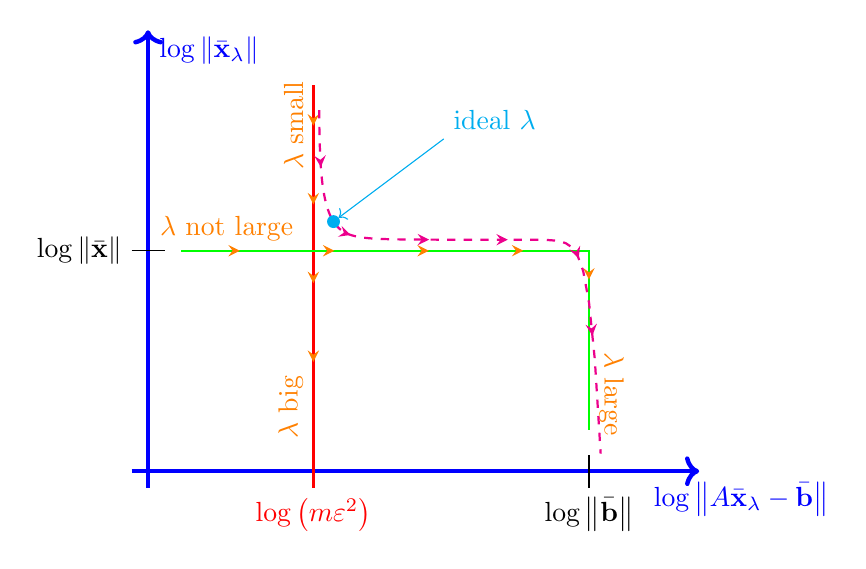
\begin{tikzpicture}[scale=0.7]
			\pgfmathsetmacro{\wth}{0.3pt}
			\draw[blue, ultra thick, ->] (-0.3,0) -- (10, 0) node[pos=0.9, below right] {$\log \left\|A\bar{\textbf{x}}_\lambda - \bar{\textbf{b}}\right\|$};
			\draw[blue, ultra thick, ->] (0,-0.3) -- (0,8) node[pos=0.9, above right] {$\log \left\|\bar{\textbf{x}}_\lambda\right\|$};
			\draw[thick, red,
				postaction={
					decorate,
					decoration={
						markings,
						mark=between positions 0.1 and 0.85 step 10mm with {\arrow[orange]{stealth};}
					}
				}] (3, 7) -- (3, -\wth) node[pos=1, below] {$\log \left(m \varepsilon^2\right)$} node[pos=0.1, orange, above, rotate=90] {$\lambda$ small} node[pos=0.8, orange, above, rotate=90] {$\lambda$ big};
				
			\draw[thick, green,
			postaction={
				decorate,
				decoration={
					markings,
					mark=between positions 0.1 and 0.9 step 12mm with {\arrow[orange]{stealth};}
				}
			}] ({2.0*\wth}, 4) -| (8, {2.5*\wth}) node[pos=0.15, orange, above left] {$\lambda$ not large} node[pos=0.9, orange, above, rotate=-90] {$\lambda$ large};
			\draw[] (-\wth, 4) -- (\wth, 4) node[pos=0, left] {$\log \left\|\bar{\textbf{x}}\right\|$};
			\draw[] (8,-\wth) -- (8,\wth) node[pos=0, below] {$\log \left\|\bar{\textbf{b}}\right\|$};
			
			\draw[magenta, dashed, thick, variable=\t,samples=100, domain=-4.7:5.8,postaction={decorate,decoration={markings,mark=between positions 0.1 and 0.8 step 10mm with {\arrow[magenta]{stealth};}}},
				]
				 plot ({3.1+ln(1+exp(\t)/2)}, {4.2+0.25*ln(1+exp(-\t*2))-3.9/ln(2)*ln(1+exp((\t-5.8))^7)}) ;
			\node[draw, circle, fill, cyan, inner sep = 1.5pt] (Lopt) at ({3.1+ln(1+exp(-0.5)/2)},
			 {4.2+0.25*ln(1+exp(0.5*2))-3.9/ln(2)*ln(1+exp((-0.5-5.8))^7)}){};
			\draw[<-, cyan] (Lopt) -- +(2,1.5) node[pos=1, above right] {ideal $\lambda$};
		\end{tikzpicture}
		\caption{L-curve theory. $m $ is the number of nonzero singular values of the matrix $A$. The errors associated to $\textbf{e}$ are in {\color{red}red}, while those linked to $\bar{\textbf{b}}$ are in {\color{green}green}. The overall behaviour belonging to $\bar{\textbf{x}}_\lambda$ is shown in {\color{magenta}magenta}} (this is the titular L curve).\label{fig:Lcurve-theory}
	\end{figure}
	
	The maximum curvature point is found automatically with the help of \textcite{Kroon_2011}.
	\FloatBarrier
	\subsection{Generalized cross-validation}
	GCV is based on the philosophy that if an arbitrary element $\mbf{b}_i$ of the right-hand side $\mbf{b}$ is left out, then the corresponding regularized solution should predict this observation well, and the choice of
	regularization parameter should be independent of an orthogonal transformation of $\mbf{b}$. This (through some complex theory that we need not worry about) leads to choosing the regularization parameter, which minimizes the GCV function
	$$G =\frac{\|A\mbf{x}_{\text{REG}} - \mbf{b}\|_2^2}{(\text{trace}(I_m - AA^I ))^2}$$
	where $A^I$ is a matrix which produces the regularized solution $\mbf{x}_{REG}$ when multiplied with $\mbf{b}$, i.e.
	$\mbf{x}_{\text{REG}} = A^I \mbf{b}$. For instance, in the case of Tikhonov regularization (with $L = I_m$ ) we have that
	$A^I = V F \Sigma^{-1}U^T$ (you can easily check this) when $A = U \Sigma V^T$ is the singular value decomposition of $A$ and $F$ is the corresponding diagonal matrix of filter factors at the parameter $\lambda$. Note that G
	is defined for both continuous and discrete regularization parameters. \textbf{Show the following, more general statement:}
	\begin{lemma}
		We have that $\text{trace}(I_m - AA^I ) = m - (n -p) - \sum_{i=1}^p f_i$
	\end{lemma}
	\begin{proof}
		The decomposition for $A$ and $A^I$ can be substituted into 
		\begin{equation}
			\text{trace}(I_m - AA^I ) = \text{trace}(I_m - U \Sigma V^T A^I V F \Sigma^{-1}U^T ) = \text{trace}(I_m - U \Sigma  F \Sigma^{-1}U^T ) = \text{trace}(I_m) - \text{trace}(F)
		\end{equation}
		where we used the orthogonality of $V, U$. $A\in\mathbb{R}^{m\times n}$ ($\textbf{x}$ is $n$, and $\textbf{b}$ is $m$ dimensional) and $B \in p \times n$. Due to \autoref{eq:tik-gsvd-sol} shows that $F$ must have $n-p$ $1$'s on its diagonal and the rest must be filled with 1's. Therefore the formula in the lemma is justified.
		\pdfmargincomment[author=Andras]{The dimensions might be a bit off here, maybe should be put in slighlty different form?}%
	\end{proof}
	 Note that for truncated algorithms the meaning of $p$ might become the number of approximating singular values used for instance. 
	 
	 For the conjugate gradient method because we are solving the normal equation $m=n$. $p$ will denote the number of iterations (the dimension of the Krylov subspace).
	 
	 
	%\textbf{What are $n$ and $p$ for CG? Assume $x_0=0$ and $A^TA$ positive definite.}
	
	
	\section{Application: the watchmaker and the bowl of soup}
	In this section we introduce a slightly silly application of the regularization methods described.
	\subsection{Context}
	Imagine you are a watchmaker, specializing in wristwatches. As such you have very sensitive hands and fingertips. In addition, you cannot allow them to be burned. Today, your partner has made you a bowl of soup, heated in the microwave and set it down at your workbench. You notice that the bowl is ceramic, which means it is probably very hot. Contrary, you deduce from the lack of steam that the soup is room temperature. Unfortunately, there is no cloth around that is thick enough to protect your hands from the scorching ceramic over the long trip back to the microwave. Fortunately though, you are skilled in integral equations and you can tell temperatures using your fingers with an accuracy of about $1e-3$ degrees. And so you put your finger in the soup, close to the bowl, but not touching, and measure the temperature as a function of time. You use this to determine the temperature of the bowl by solving \emph{the inverse heat equation.}
	\subsection{The inverse heat equation}
	We model this as the inverse of the following heat equation:
	\begin{align*}
		\frac{\partial}{\partial t}T\,\,\,&=\frac{\partial^2}{\partial^2x}T\\
		T(x,0)&=\,\,0\\
		T(0,t)&=f(t)
	\end{align*}
	for $0<x<\infty$ and $0\leq t<\infty$.
	Here, the temperature $T = 0$ actually corresponds to room temperature, that is $20$ degrees Celsius. The origin ($x=0$) corresponds to the bowl. The variable $t$ in our example is measured in minutes. By inverse we mean: while the above calculates $T$ given the boundary condition $f$ , we wish to compute $f$ from the observed $T(y, t) := g(t)$ at a distance y from the origin. It is known that this is given by
	$$Kf=g$$
	with
	$$(Kf)(t)=\frac{y}{2\sqrt{\pi}}\int_0^t\frac{f(\xi)}{(t-\xi)^{3/2}}\exp(\frac{-y^2}{4(t-\xi)})\,d\xi.$$
	This is a Volterra integral equation, but can be transformed into a Fredholm equation by extension. It is thus immediately suspect: the discretization of this problem is probably ill-posed.
	\subsection{Provided data}
	You have been provided a matrix $K$, obtained by the mid-point rule discretization of the operator
	$K$. In addition you are given an exact solution $f$ and a perturbed (random normally distributed noise, $\sigma = 1e-3$) right-hand-side $\mathbf{g}$. Both are given over a time range of
	$10$ minutes.
	\subsection{Extra information about the solution}
	Since regularization is all about using information about the solution, some information is provided that could be used . You can verify this by looking at the exact solution given. %\textbf{Not every piece of information needs to be used, or might even be helpful!}
	\begin{itemize}
		\item[(1)] The solution is not oscillatory. This can be achieved by requiring that its second derivative is
		small
		\item[(2)] The solution is eventually zero. In fact, if $t > 5$, $f$ is negligible
		\item[(3)]The temperature is always positive i.e. $f > 0$
		\item[(4)]Initially, the temperature is stationary, that is, $g'(0) = 0$
	\end{itemize}
	
	\subsection{Solution}
	The condition number of the matrix $A$ (\texttt{K} variable in MATLAB) is indeed quite unfavourable, calculated to be \texttt{4.9151e+124}. 
	\begin{table}
		\begin{tabular}{|c||c|c|c|c|c|c|c|c|}
			\minput{../codes/test.txt}
		\end{tabular}
	\end{table}
	
\FloatBarrier
\pagebreak
\printbibliography
\end{document}